\section{Resultados e Discussão}
\label{sec:resultados}

Esta seção apresenta os resultados nas duas etapas. Primeiro, o desempenho preditivo do modelo
hedônico e sua comparação com a \textit{baseline}. Em seguida, o resultado causal central: a
correlação ingênua entre liquidez e sobrepreço desaparece sob \textit{Double Machine Learning}, mas
um efeito significativo emerge em temporadas específicas. Por fim, a heterogeneidade entre clubes e
uma bateria de testes de robustez.

\subsection{Desempenho do modelo hedônico}

A Tabela~\ref{tab:hedonico} compara os quatro modelos com a \textit{baseline}, que prevê o
\textit{fee} usando apenas o valor de mercado. Todos os modelos superam a \textit{baseline}, e o
\textit{Random Forest} obtém o melhor desempenho no \textit{holdout} de 2025, com $R^2 = 0{,}762$ e
RMSE de $0{,}673$ — um ganho de \textbf{7,4 pontos percentuais} de $R^2$ sobre a \textit{baseline}
($0{,}688$). O pequeno desvio entre validação cruzada e teste indica ausência de sobreajuste
relevante.

\begin{table}[ht]
\centering
\caption{Desempenho preditivo no \textit{holdout} de 2025 (alvo: $\log$ do \textit{fee}).}
\label{tab:hedonico}
\begin{tabular}{lcc}
\toprule
\textbf{Modelo} & \textbf{Test RMSE} & \textbf{Test $R^2$} \\
\midrule
\textit{Baseline} (só valor de mercado) & 0,769 & 0,688 \\
XGBoost                                  & 0,692 & 0,748 \\
LightGBM                                 & 0,683 & 0,754 \\
\textbf{Random Forest}                   & \textbf{0,673} & \textbf{0,762} \\
SVR (RBF)                                & 0,716 & 0,730 \\
\bottomrule
\end{tabular}
\end{table}

A análise de importância por valores SHAP \cite{lundberg2017} confirma que o valor de mercado é, de
longe, o principal preditor do \textit{fee}, seguido por idade e liga — validando empiricamente a
premissa hedônica. O resíduo resultante (o sobrepreço de reinvestimento) tem média próxima de zero
por construção, mediana de \textbf{+3,5\%} e desvio-padrão de $0{,}671$; \textbf{52,5\%} das
transferências situam-se acima do preço justo estimado. É sobre esse resíduo que a análise causal se
debruça.

\subsection{Da correlação à causa: o efeito médio}

A Figura~\ref{fig:estimadores} resume o resultado central. Uma regressão ingênua do sobrepreço
contra a liquidez, \textbf{sem controles}, estima um efeito positivo e significativo
($\theta = 0{,}0142$; IC~95\% $[0{,}0092;\,0{,}0192]$) — a evidência aparente de um ``prêmio do
vendedor''. Contudo, ao introduzir os confundidores estruturais, o efeito encolhe pela metade
($\theta = 0{,}0051$) e perde significância. Sob \textit{Double Machine Learning}
\cite{chernozhukov2018}, que controla os confundidores de forma flexível, o efeito médio é de apenas
$\theta = 0{,}0044$, com intervalo de confiança que cruza zero tanto com erros-padrão robustos
($[-0{,}0016;\,0{,}0104]$) quanto clusterizados por clube e temporada
($[-0{,}0021;\,0{,}0110]$). \textbf{O efeito causal médio é, portanto, estatisticamente nulo.}

\begin{figure}[ht]
\centering
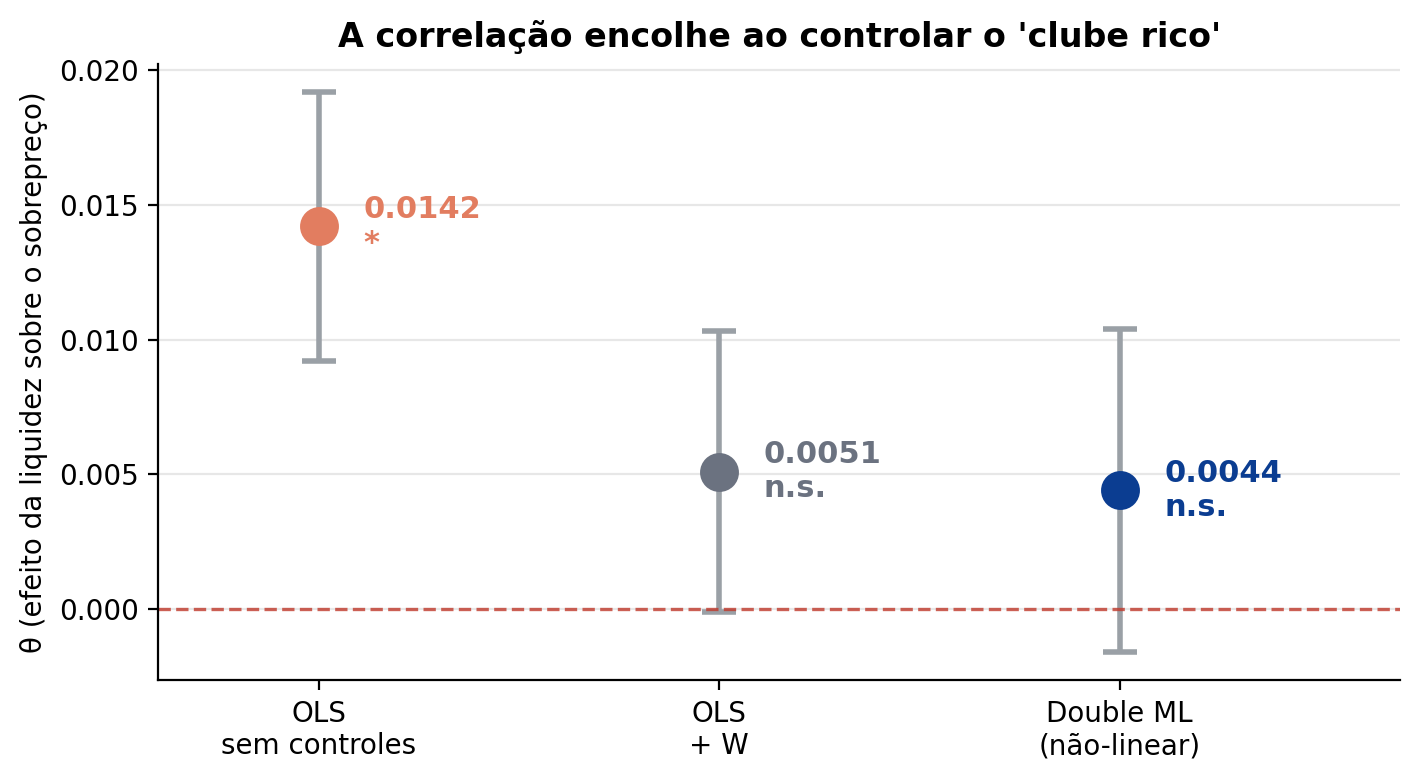
\includegraphics[width=0.7\linewidth]{imgs/comparacao_estimadores.png}
\caption{Estimativas do efeito da liquidez sobre o sobrepreço sob três especificações. A correlação
ingênua (OLS sem controles) é positiva e significativa, mas encolhe e perde significância ao
controlar os confundidores (OLS + W) e sob DML. As barras indicam o IC de 95\%.}
\label{fig:estimadores}
\end{figure}

Dois testes \textit{placebo} confirmam a validade do desenho: ao substituir o tratamento por uma
permutação aleatória ($\theta = 0{,}0024$) ou por ruído gaussiano ($\theta = 0{,}0009$), o efeito
estimado é indistinguível de zero — o modelo não detecta efeito espúrio. Note-se que o
\textit{placebo} permutado tem magnitude próxima à do efeito real, coerente com a nulidade do efeito
médio. O diagnóstico de primeira etapa mostra que os confundidores preveem moderadamente o
tratamento ($R^2 = 0{,}37$) e pouco do resíduo ($R^2 = 0{,}06$), este último esperado, já que $Y$ já
é um resíduo depurado dos atributos do jogador.

\textbf{Interpretação.} A correlação ingênua era, em grande parte, o confundidor ``clube rico'' em
ação: clubes que vendem caro também compram caro por serem financeiramente robustos, não porque a
venda os torne reféns do mercado. Sem o controle causal, concluiríamos erroneamente pela existência
de um prêmio do vendedor sistemático.

\subsection{Onde o efeito vive: heterogeneidade temporal}

A nulidade média, porém, esconde forte heterogeneidade no tempo. A Figura~\ref{fig:sazonal} mostra o
efeito estimado por temporada. De 2017 a 2021 e em 2024--2025, o efeito é indistinguível de zero.
Em \textbf{2022} ($\theta = 0{,}064$; $p = 0{,}0006$) e \textbf{2023} ($\theta = 0{,}047$;
$p = 0{,}0024$), contudo, o prêmio do vendedor é positivo e significativo — e, crucialmente,
\textbf{ambos sobrevivem à correção de Bonferroni e ao controle de \textit{false discovery rate}}
\cite{benjamini1995} para os oito testes sazonais, afastando a hipótese de falso-positivo por
testagem múltipla.

\begin{figure}[ht]
\centering
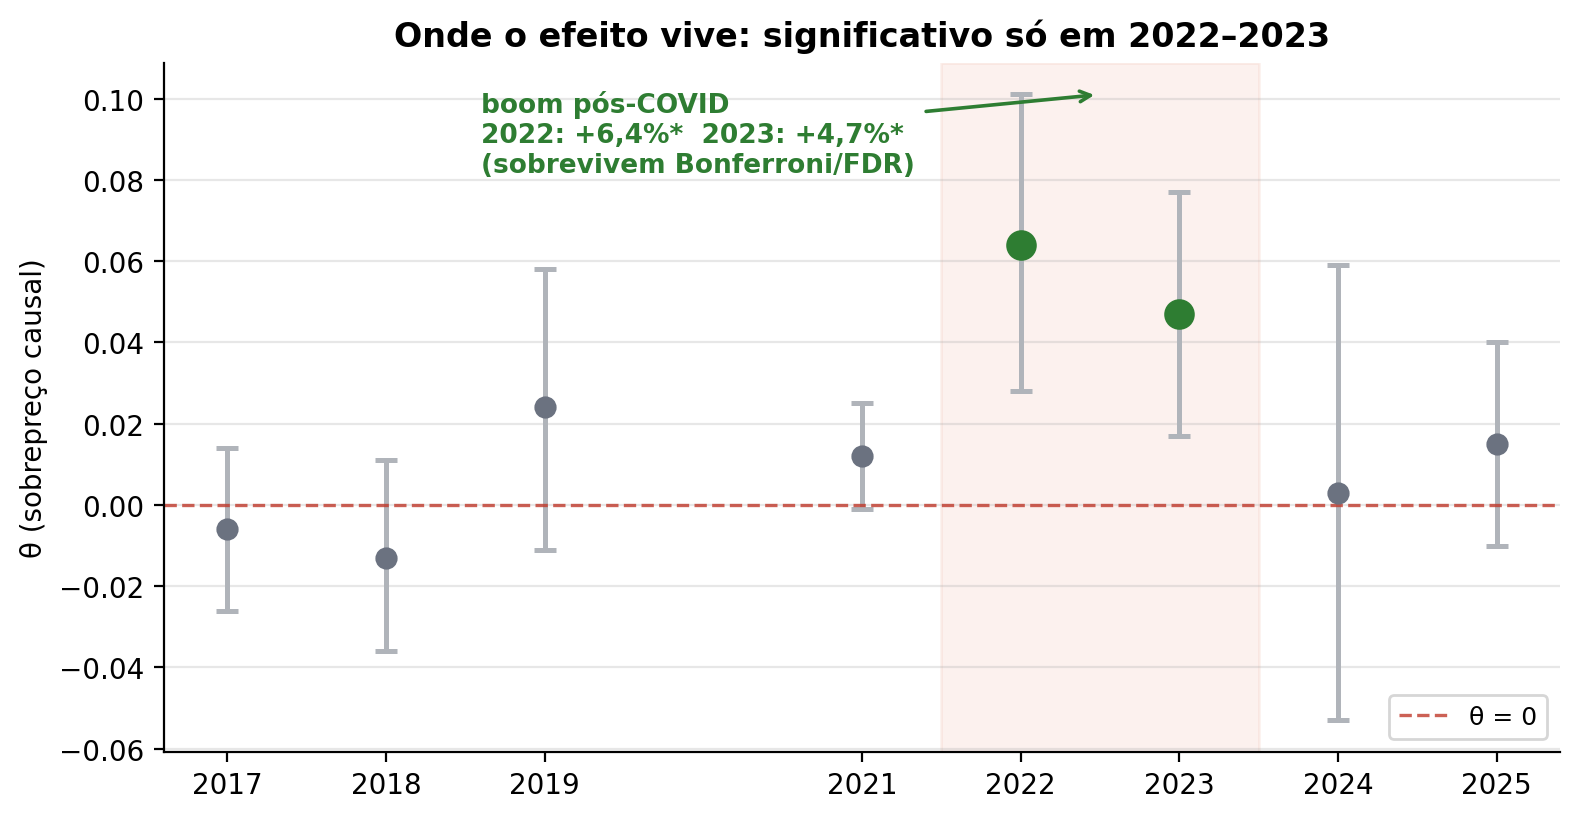
\includegraphics[width=0.8\linewidth]{imgs/theta_sazonal.png}
\caption{Efeito causal da liquidez sobre o sobrepreço, estimado por temporada (IC de 95\%
clusterizado). O efeito é nulo na maioria dos anos e significativo apenas em 2022 e 2023, no auge da
recuperação de mercado pós-pandemia.}
\label{fig:sazonal}
\end{figure}

Esses são justamente os anos do \textbf{boom de mercado pós-COVID}, quando o volume de transferências
atingiu níveis recordes após duas temporadas de retração. Nesse regime de mercado aquecido — com
escassez de alvos disponíveis e urgência de reposição — clubes capitalizados de fato pagam mais. O
achado central deste trabalho é, portanto, que \textbf{o prêmio do vendedor não é uma lei universal
do mercado, mas um fenômeno condicional ao regime}. Análises de janelas curtas (como a de três
temporadas usada em iterações anteriores deste projeto) podem capturar espuriamente um efeito médio
significativo ao concentrarem-se em anos atípicos.

\subsection{Heterogeneidade entre clubes: o IVB}

Estendendo a análise ao nível de clube, o \textit{R-learner} \cite{nie2021} estima um efeito
condicional por transferência, agregado por clube comprador no \textit{Índice de Vulnerabilidade de
Barganha} (IVB). Conceitualmente, o IVB ordena clubes entre ``presas fáceis'' (que pagam mais
sobrepreço quando capitalizados) e ``negociadores disciplinados''. \textbf{Este resultado deve ser
lido com cautela}: os efeitos condicionais têm baixo poder estatístico ($R^2$ de primeira etapa do
desfecho de apenas $0{,}06$) e o ordenamento é sensível a clubes com poucas transações, sendo o topo
do \textit{ranking} dominado por um \textit{outlier}. Tratamos o IVB, portanto, como uma
\textbf{demonstração de conceito exploratória} — uma direção promissora para inteligência de
mercado (Seção~\ref{sec:aplicacoes}), não como um resultado conclusivo.

\subsection{Robustez}

Submetemos o achado a uma bateria de testes, sintetizada na Tabela~\ref{tab:robustez}. O efeito
sazonal de 2022--2023 mostra-se robusto: um \textit{placebo} de permutação intra-safra produz
$p$ empírico de $0{,}005$; o efeito é estável a variações do limiar de \textit{fee} (de €0 a €1M); e
o \textit{Robustness Value} \cite{cinelli2020} de $\approx 0{,}24$--$0{,}27$ indica que um
confundidor omitido precisaria explicar cerca de um quarto da variação residual do tratamento
\textit{e} do desfecho para anular o efeito. Mesmo num teste de \textit{over-control}, que
reintroduz o volume financeiro no vetor de confundidores, o efeito de 2023 sobrevive
($p \approx 0{,}003$), embora o de 2022 atenue.

Dois resultados qualificam a interpretação. O \textbf{teste de tratamento defasado} (liquidez da
temporada anterior) é significativo ($\theta = 0{,}0051$), o que enfraquece a hipótese de
causalidade reversa; porém, como o efeito contemporâneo na mesma subamostra é não significativo, o
teste \textbf{não é conclusivo}. Especificações alternativas do tratamento — número de vendas e
indicador de venda de grande porte — são significativas isoladamente ($\theta = 0{,}049$ e
$0{,}075$), sugerindo um mecanismo de ``sinalização de necessidade''; entretanto, ao controlar a
intensidade de atividade do clube, ambas perdem significância, de modo que esse mecanismo permanece
como \textbf{hipótese exploratória}, não como achado confirmado.

\begin{table}[ht]
\centering
\caption{Síntese da bateria de robustez.}
\label{tab:robustez}
\begin{tabular}{lll}
\toprule
\textbf{Teste} & \textbf{Resultado} & \textbf{Leitura} \\
\midrule
\textit{Placebo} (permutação / ruído)      & $\theta \approx 0{,}002$ / $0{,}001$ & desenho não gera efeito espúrio \\
Bonferroni / FDR (8 testes sazonais)        & 2022 e 2023 sobrevivem & efeito sazonal não é falso-positivo \\
\textit{Placebo} permutação intra-safra     & $p_{emp} = 0{,}005$ & efeito de 2022--2023 é real \\
Sensibilidade ao limiar de \textit{fee}     & estável (€0--€1M) & não é artefato do corte \\
\textit{Robustness Value}                   & $0{,}24$--$0{,}27$ & confundidor omitido teria de ser forte \\
\textit{Over-control} (com volume financeiro)& 2023 sobrevive ($p\approx0{,}003$) & robusto a controle financeiro direto \\
Tratamento defasado (C2)                     & $\theta = 0{,}0051$ (não conclusivo) & causalidade reversa enfraquecida \\
Tratamentos alternativos (vendas / porte)    & signif.\ isolado, n.s.\ com controle & mecanismo exploratório \\
\bottomrule
\end{tabular}
\end{table}
